%%%%%%%
%%%%%%%
%%%%      SECTION HEADING
%%%%%%%
%%%%%%%

We follow the notation and terminology laid out in the ``sparkstruck preliminaries" document in this project's ``background-reading" subdirectory.

Let $G$ be a standard, connected graph with adjacency matrix $\mA$. A graph is \emph{walk-regular} iff the diagonals of the powers of $\mA$ are each constant, i.e. for all $k$ we have $\diag( \mA^k ) = b_k \mI$ where for each $k$, $b_k$ is a constant. Intuitively this property means that at every length of walk $k$, every node in the graph has the same number of closed walks of length $k$. This is one sense in which a graph can be ``kind of uniform", i.e. have all nodes ``look the same". (This is distinct from the property of a graph being \emph{vertex transitive}, i.e. each node has the exact same structural property as all other nodes. Vertex transitivity is a very strict notion of node regularity -- walk-regularity is not quite as strict.)


A question central to this project is the following: given a graph $G$ and a function $f(x)$ with mild assumptions, when does the condition ``$\diag( f(\mA) )$ is a constant" imply that the graph $G$ is walk-regular? (i.e. what properties of the graph, and what properties of the function are sufficient to guarantee that statement works out?)

This originates from a conjecture of Michele Benzi's, which states that ``for any $f(x)$ with power series representation $f(x) = \sum_{k=0}^{\infty} c_k x^k$ with $c_k > 0$, if $\diag( f(\mA) )$ is constant then the graph is walk regular."
We know that a statement even stronger than the converse is true: if $G$ is walk regular, then for \emph{any} function $f$ we have that $\diag(f(\mA))$ is a constant.
Some progress has been made on the forward direction: Estrada and de la Pena showed in~\cite{estrada2014maximum} that for the specific function $f(x) = \exp(x)$ we have that ``if $\diag(\exp(\mA))$ is a constant, then $G$ is walk-regular".

However, Blair and I were able to construct a counter example to Benzi's original conjecture: we present a function $f$ satisfying Benzi's positivity property and a graph (Figure~\ref{fig:counterexample-dreidel}) that is \emph{not} walk-regular, yet the diagonal $\diag(f(\mA))$ is a constant. We call such a function ``deceptive with respect to $G$". To continue the flavor of this terminology, we would say that $\exp$ is an \emph{honest} function, since $\diag(\exp(\mA))$ being constant implies $G$ is walk-regular for \emph{any} graph $G$.

\subsection{Description of this project}
This project focuses on determining: are there classes of graphs for which all positive-power-series functions are honest? Are there classes of function that are honest with respect to all graphs? Are there \emph{straight-forward} families of graphs for which we can always construct deceptive functions?

\begin{figure}[ht]
\centering
%\hspace{1em}
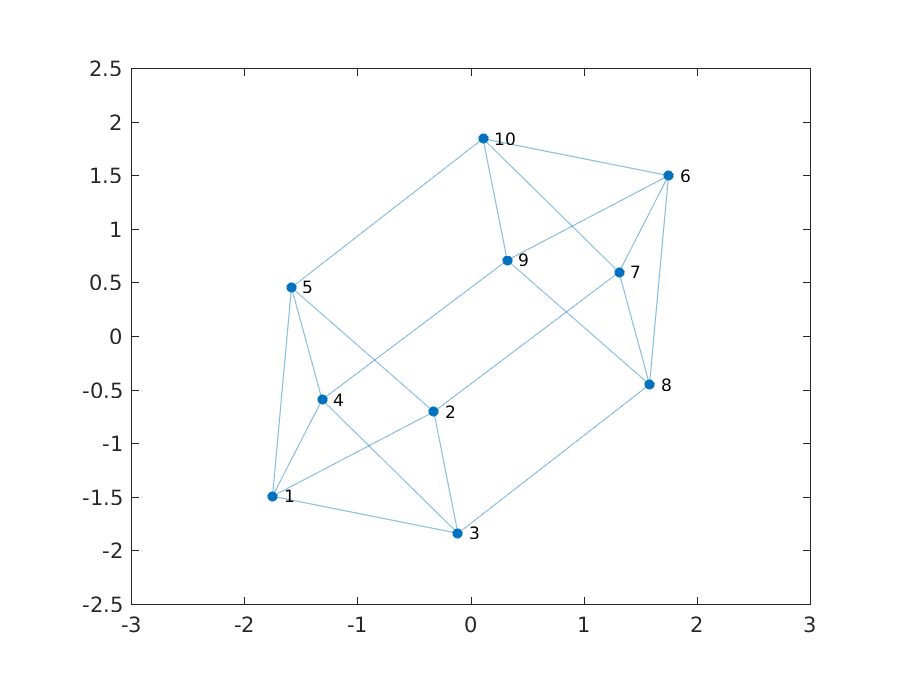
\includegraphics[width=0.7\linewidth]{walk-counterexample}%
%\hspace*{1em}
\caption{We have constructed a deceptive function for this graph, i.e. a function with constant diagonal $\diag(f(\mA))$, even though this graph is not walk-regular.}
\label{fig:counterexample-dreidel}
\end{figure}

To begin answering these questions, we first focus on some simple, individual cases. The counter-examples that Blair and I have discovered so far are all graphs with exactly two ``walk-classes" (i.e. groups of nodes with identical values in $\diag(\mA^k)$ for all $k$ ).
This setting makes it much clearer whether or not a deceptive function can be constructed.
We were able to prove that, for any non--walk-regular graph $G$ with exactly two walk-classes, a function $f$ that is deceptive with respect to $G$ can be constructed iff the two classes ``flip-flop" -- that is, if there exists one walk-length $L_1$ of which class A has more walks than class B, and a second walk-length $L_2$ of which class A has fewer walks than class B. (We make this more precise below.) For any such 2-class, non--walk-regular graph we give an explicit construction of a function that is deceptive with respect to $G$.

%We hope to generalize our counter-example construction to the case that the graph has $k$ distinct walk-classes. We have a sufficient condition (i.e. a condition on the ``flip-flopping" of the $k$ distinct node classes that is sufficient to guarantee the existence of a function that is deceptive on $G$) but we are not sure if the condition is also necessary.
